\سؤال{}

\textbf{با توجه به مباحثی که در فصل‌های \lr{Design} آموخته‌اید، نرم‌افزار را طراحی نمایید.}

تفاوت اصلی بخش تحلیل و طراحی مربوط به قلمرو آن‌ها است. همان‌طور که در سوال «۷» گفتیم، محدوده‌ی تحلیل در قلمرو مسئله و محدوده‌ی طراحی در قلمرو جواب ‌\footnote{\lr{solution domain}} است. این بدان معنی است که جزئیات فنی نیز در این بخش مانند پایگاه‌داده، تکنولوژی‌های مورد استفاده و... در نظر گرفته می‌شوند.

نمودارهای زیادی در بخش طراحی وجود دارند:
\begin{itemize}
	\item نمودار کلاس با جزئیات فنی
	\item نمودار مستقرسازی\footnote{\lr{deployment diagram}}
	\item نمودار مؤلفه \footnote{\lr{component diagram}}
	\item نمودار توالی \footnote{\lr{sequence diagram}}
	\item و...
\end{itemize}

با توجه به محدودیت زمان امتحان، تصمیم گرفته‌ام تا نمودار کلاس را تا حد امکان ساده و کاربردی پیاده‌سازی کرده و وارد جزئیات بیش از حد نشوم.
\begin{itemize}
	\item \textbf{ نمودار کلاس}
	
	\begin{figure}
		\begin{center}
			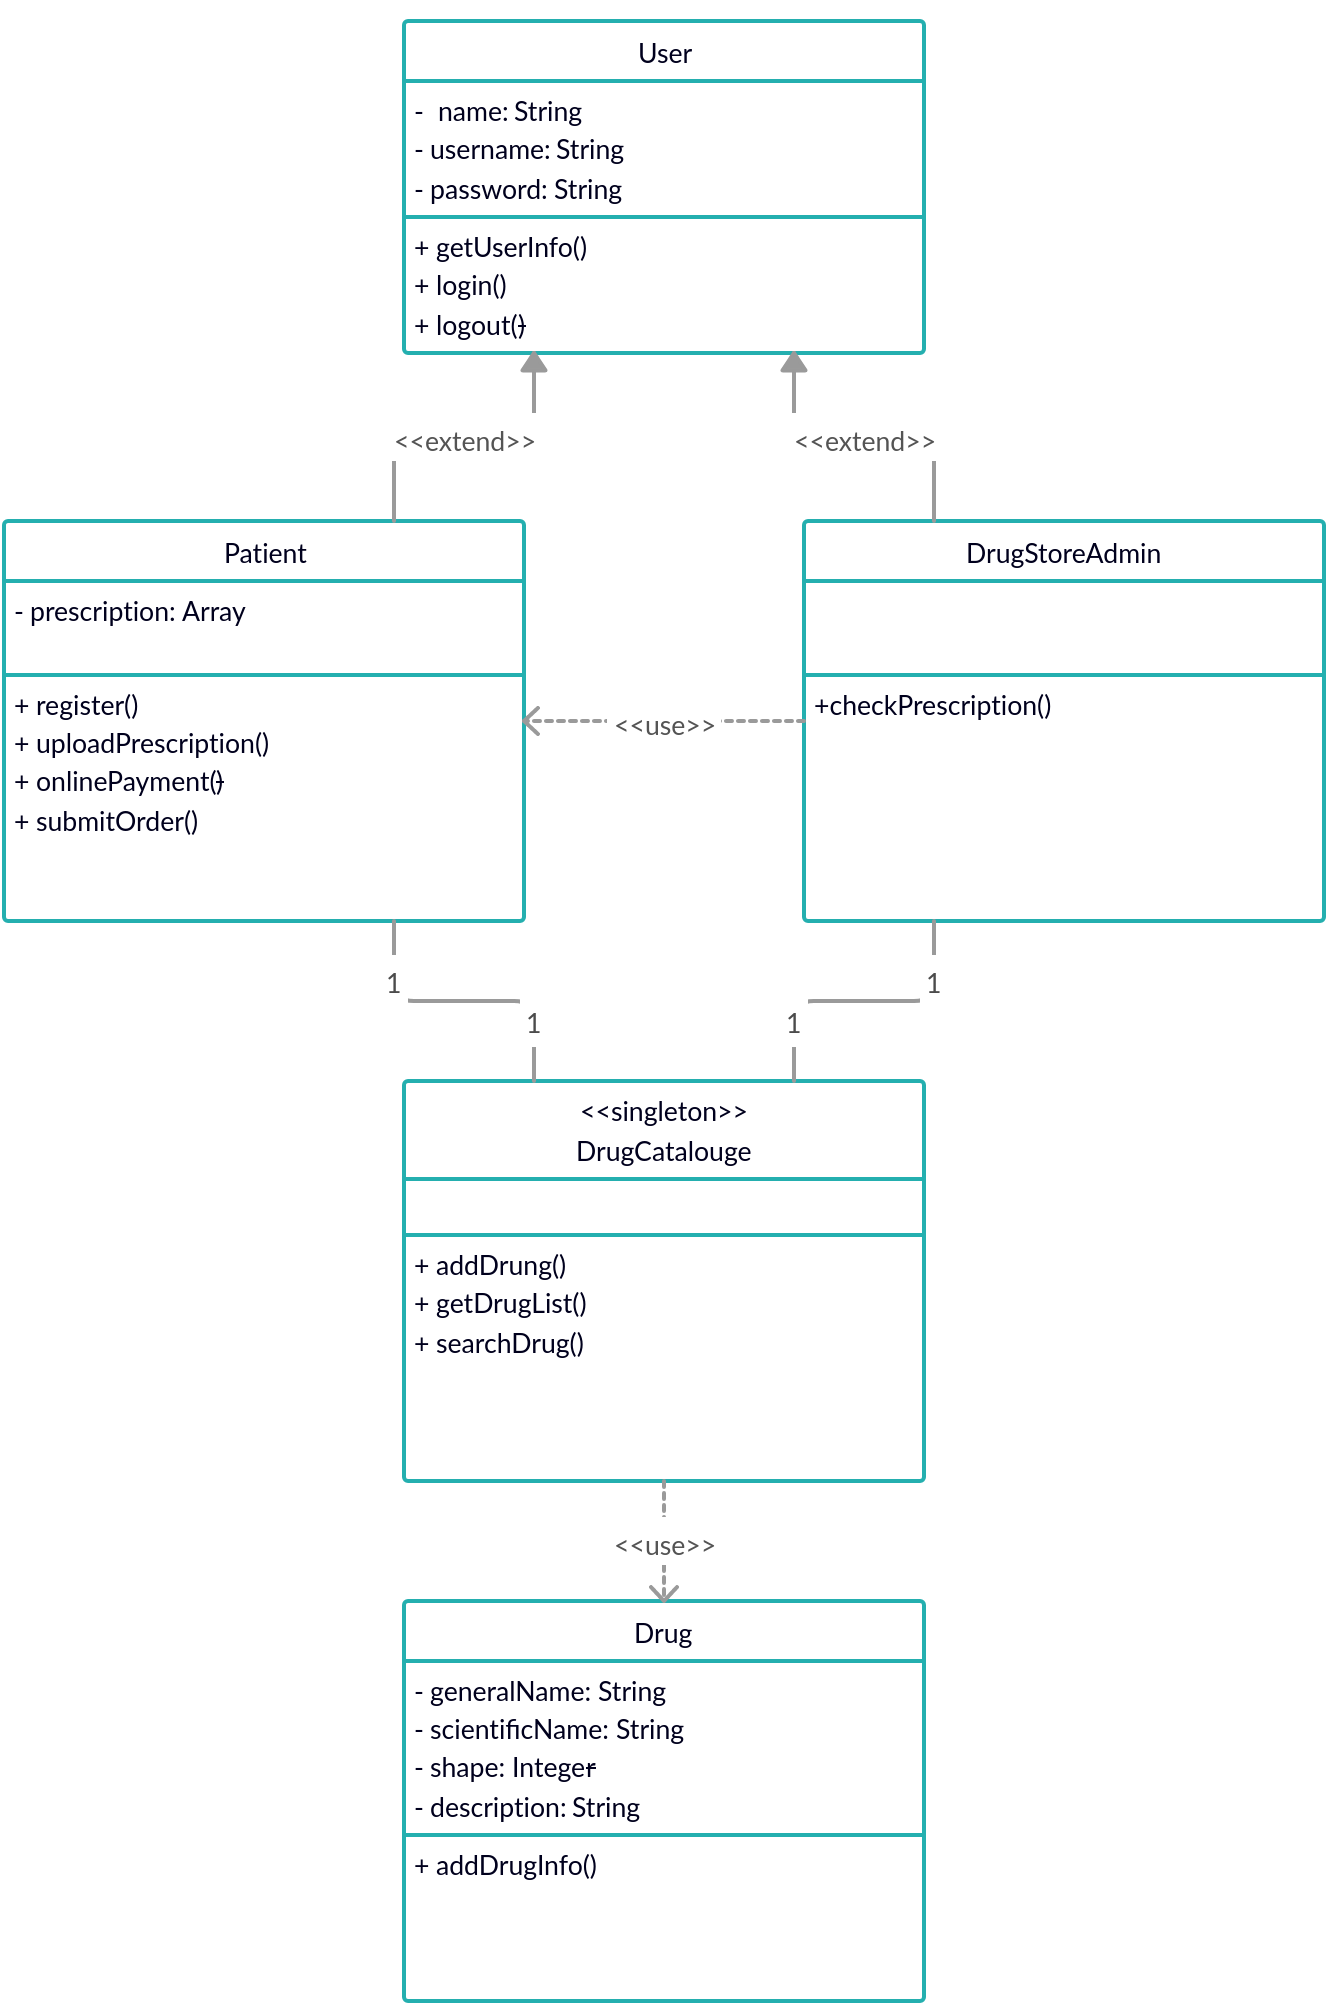
\includegraphics[scale=0.3]{./8.png}
			\caption{نمودار کلاس بخش طراحی}
		\end{center}
	\end{figure}
\end{itemize}